
\chapter{The transmission of the Welsh laws}
\label{cha:welsh-laws}

\section{Some quotes, tables, and stemmas}
\label{sec:some-quotes-tables}


% \tqt{One advantage which Welsh law enjoyed in the political storms of the thirteenth century was that it had a written form. Already in the twelfth century it was felt to be an embarassment if law remained unwritten. Roman law was embodied in texts, and with the great legal revival of the eleventh and twelfth centuries it was felt that any law worthy of the name should be written.
% }{charles-edwards_welsh_1989}{14}

\tqt{Welsh law survives in many complete manuscripts and fragments of others. The difficulty scholars have had in coping with this wealth of material stems from two opposite truths: first, each manuscript is an individual entity in that no one manuscript presents a text exactly the same as any other; but, secondly, the manuscripts fall into groups because they share, to a greater or lesser extent, the same content. As a result there have been long terminological travails attempting to give due weight both to the variations between manuscripts and also the links between them.
}{charles-edwards_welsh_1989}{17}


\tqt{The considerable differences between the law books show that their authors were not concerned, like the Irish, to preserve intact a standard text handed down from the past.
  Linguistically, the laws are not unlike many Middle Welsh prose tales: in spite of the occasional early feature the language as a whole generally accords with the dates of the manuscripts.
}{charles-edwards_welsh_1989}{21--22}

% \tqt{{[T]}he distinction between the Versions and the Anomalous Laws lies in the existence of a certain pattern according to which it was thought that a wide-ranging account of the Law of Hywel ought to be constructed. The pattern was not immutable, as is shown by the creation of the Test Book in \textsc{Ior} or by the wide variations in the ordering of the tractates in \textsc{Cyfn}.}{charles-edwards_welsh_1989}{26}

\Textcite{wiliam_llyfr_1960} notes that, within \textit{B}, `[m]utations of initial consonants are sometimes indicated, sometimes not. The nasal mutation, however, is regularly shown.'~\autocite[xlii]{wiliam_llyfr_1960}.

\begin{figure}[h]
  \centering
  \begin{tikzpicture}[font=\itshape,level distance=10mm]
    \node(A){A}
    child {node {E}
      child [missing]
      child [missing]
      child {node(B) {B}}
    }
    child [missing]
    child {node(C) {C}}
    ;
    \draw(B)--(C)
    ;
    \node[right= 1em of C](S){\upshape saec.~XIII\textsuperscript{med}};
    \node[right= 5em of A]{c.~\upshape 1200};
    \node[right= 5em of B]{c.~\upshape 1282};
  \end{tikzpicture}
  \caption{Gwenogvryn Evans's \mw{Llyfr Iorwerth}}
  \label{fig:gwevanslli}
\end{figure}

\begin{figure}[h]
  \centering
  \begin{tikzpicture}[font=\itshape]
    \node{X}
    child {node(alph) {α}
      child {node(B) {B}}
    }
    child {node (beta) {β}
      child {node(C) {C}}
      child {node (gamma) {γ}
        child {node (delta) {δ}
          child{node{A}}
          child{node{E}}
        }
        child[missing]
        child {node (eps){ε}
          child {node{D}}
          child{node{ζ}
            child {node {Col}}
            child {node {\upshape Llanforda}}
          }
        }
      }
    }
    ;
    \node[left=of alph](nalph){Galanas B \upshape added};
    \node[left= of B](nB){{\upshape no} damweiniau};
    \node[below left= of C](nC){{\upshape no} damweiniau};
    \node[below left=of delta,align=left](ndelta){- {\upshape Pref.\ to Test Bk.}\\+ Br.\ Gwŷr Arfon};
    \node[right=of beta](nbeta){+ Galanas E \upshape\& Pref.\ to Test Book};
    \node[right=of gamma](ngamma){+ Damweiniau I};
    \node[right=of eps](neps){+ Damweiniau II};
    \draw[dotted](alph)--(nalph);
    \draw[dotted](B)--(nB);
    \draw[dotted](C)--(nC);
    \draw[dotted](delta)--(ndelta);
    \draw[dotted](beta)--(nbeta);
    \draw[dotted](gamma)--(ngamma);
    \draw[dotted](eps)--(neps);
  \end{tikzpicture}
  \caption{Wiliam's \mw{Llyfr Iorwerth}, simplified by Thomas Charles-Edwards.}
  \label{fig:wiliamiorwerth}
\end{figure}

%  \begin{figure}[h]
%     \centering
% \begin{tikzpicture}[font=\itshape]
% \node{\upshape Redaction I} 
% child {node {α}
%   child [level distance=15mm]{node {A}}
%   child [level distance=15mm]{node {E}}
% }
% child [xshift=1em]{node {\upshape Redaction II}
%   child [grow=down] {node {β}
%     child [level distance =10mm,xshift=-1em]{node {C}}
%     }
%     child[level distance=20mm] {node{γ}
%       child [level distance=15mm]{node {\vphantom{J}GDLew}}
%       child [level distance=15mm]{node{BJKTim}}
%     }
% }
%     ;
%   \end{tikzpicture}
%     \caption{A stemma of the Laws of the Country  according to Thomas Charles-Edwards.}
%     \label{fig:stemmalawc}
%   \end{figure}
  
  \begin{figure}[h]
    \centering
    \begin{tikzpicture}[font=\itshape]
\node(1){\upshape Redaction I} 
child {node {α}
  child{node(A) {A}}
  child{node(E) {E}}
  child[missing]
}
child[missing]
child {node(2) {\upshape Redaction II}
  child {node[align=center] {β\\Bees I}
    child [dashed,level distance=30mm]{node(B) {B}
      edge from parent node [above,sloped]{Test Book}}
    child {node {C}}
    child[missing]
  }
  child[missing]
  child {node[align=center](gamma){γ\\Bees II}
    child  {node {GDLew}}
    child[missing]
      child [level distance=30mm]{node {JKTim}
      edge from parent node (J){}  
      }
  }
 }
  ;
  \node[above left=of E](nA){Bees I \& II};
  \node[right=of 1](n1){Bees I \& II};
  \node[right=of 2,align=center](n2){+ Preface to Test Book\\ Bees I \& II};
  \node[right=of gamma](ngamma){+ Hywel to Rome};
  \draw[dotted](A)--(nA) -- (E);
  \draw[dotted](1)--(n1);
  \draw[dotted](2)--(n2);
  \draw[dotted](gamma)--(ngamma);
  \draw[dashed](B) to  node [midway,below,sloped]{Laws of Country}  (J);
\end{tikzpicture}
\caption{A stemma of \mw{Llyfr Iorwerth} manuscripts according to Thomas Charles-Edwards. Dashed lines represent partial transmission.}
\label{fig:stemmatestb}
\end{figure}


%%% Local Variables:
%%% mode: latex
%%% TeX-master: "../main"
%%% End:


\begin{figure}[h]
  \centering
  \begin{tabular}{cc}
I  & II\\
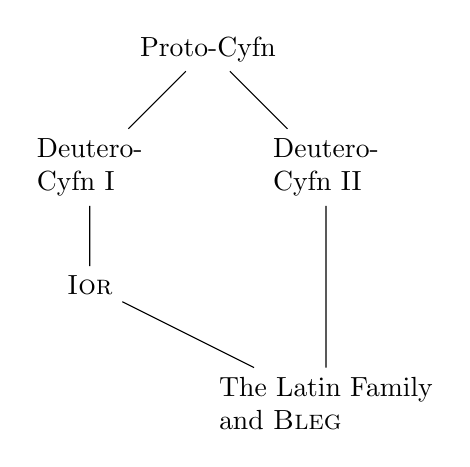
\begin{tikzpicture}[level distance=15mm,align=left]
\node(p){Proto-Cyfn}
child{node {Deutero-\\Cyfn I}
  child{node(ior){\textsc{Ior}}}
}
child[missing]
child {node {Deutero-\\Cyfn II}
  child[level distance=30mm] {node(lat){The Latin Family\\ and \textsc{Bleg}}}
}
;
\draw(ior)--(lat);    
\end{tikzpicture}
   &
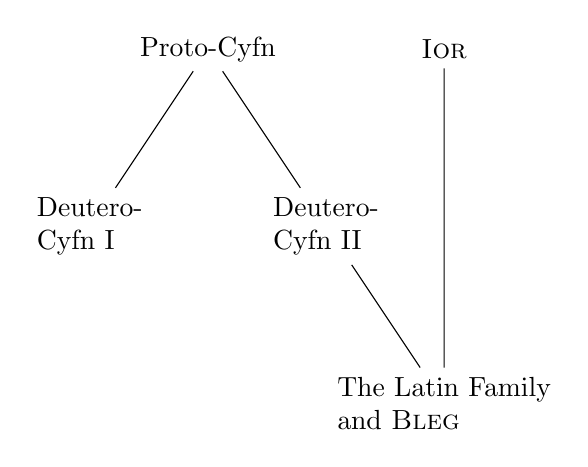
\begin{tikzpicture}[level distance=22.5mm,align=left]
\node(p){Proto-Cyfn}
child{node {Deutero-\\Cyfn I}
}
child[missing]
child {node {Deutero-\\Cyfn II}
  child[xshift=15mm] {node(lat){The Latin Family\\ and \textsc{Bleg}}}
}
;
\node[xshift=30mm](ior){\vphantom{J}\textsc{Ior}};
\draw(ior)--(lat);
\end{tikzpicture}
\end{tabular}

\caption{Two possible family trees of the Welsh law books according to \textcite[48]{charles-edwards_welsh_1989}.}
\label{fig:lawfamilies}
\end{figure}

% \begin{table}[h]
%   \centering
%   \begin{tabular}{@{}ll@{}}
%     \toprule
%     \tch{Old} & \tch{New} \\
%     \midrule
%     Ɛ & Ep \\
%     Ð & Dd \\
%     Ā & As\\
%     \rotatebox[origin=c]{180}{ω}& Mor\\
%      & An \\
%     \bottomrule
%   \end{tabular}
% \caption{Sigla for the anomalous laws}
% \label{tab:sigla}
% \end{table}

\begin{table}[h]
\centering
  \renewcommand{\labelenumi}{\Roman{enumi}}
  \renewcommand{\labelenumii}{\arabic{enumii}}
  \renewcommand{\labelenumiii}{(\roman{enumiii})}
\begin{tabular}{@{}p{0.45\textwidth}p{0.45\textwidth}@{}}
  \toprule
  \tch{\itshape Mk:}&\tch{\textsc{Ior}:}\\\midrule
\begin{enumerate}
\item Prologue
\item Laws of Court
\item Laws of Country
  \begin{enumerate}
  \item The Three Columns of Law, the Nine Tongued-ones, the value of limbs, \mw{galanas} and \mw{sarhaed}
  \item Land
  \item Value of Wild and Tame
  \item Other Laws of Country
    \begin{enumerate}
    \item Corn-damage
    \item Suretyship
    \item Women
    \end{enumerate}
  \end{enumerate}
\item Triads
\end{enumerate}
&

\begin{enumerate}
\item Prologue
\item The Book of the Court (43/17 from Manuscript \textit{B})
\item The Laws of Country
  \begin{enumerate}
  \item The Nine Tongued-ones
  \item Women
  \item Injury to Animals
  \item Surety and Contract
  \item Church Protection
  \item Land
  \item Children and Paternity
  \end{enumerate}
\item The Test Book (colophon: 120/7)
  \begin{enumerate}
  \item The Three Columns of Law (colophon: 120/7)
  \item Value of Wild and Tame (and the Value of Trees)
  \end{enumerate}
\item Appendages to the Test Book:
  \begin{enumerate}
  \item Value of Houses and Equipment
  \item Joint-ploughing
  \item Corn-damage
  \end{enumerate}
\end{enumerate}\\\bottomrule
\end{tabular}
\caption{The main divisions of \textit{Mk} and \textsc{Ior} according to \textcite[27--28]{charles-edwards_welsh_1989}}
\label{tab:divisions}
\end{table}

\section{Research plan for the laws}
\label{sec:research-plan-laws}

What do I want to do?
I want to analyze where \lT\ was represented in the various law texts.

Why do I want to do this?
I want to see under what circumstances scribes copying manuscripts maintained or changed the non-representation of \lT.

Which period is suitable for this purpose?
I expect that most instances of \lT\ were represented by the mid-fourteenth century, so manuscripts up until this period are most useful to chart the change in orthography.
Later manuscripts may still show traces of the early orthography, and may thus also be included.
I will focus on the transmission of \mw{Llyfr Iorwerth}, because most of the oldest law manuscripts contain this law text.

How are various manuscripts related to each other?
It is nowadays thought that none of the earliest extant manuscripts is a direct ancestor of another extant copy.
One author who did think this was J.\ Gwenogvryn Evans (Figure~\ref{fig:gwevanslli}).
Rather, extant manuscripts are held to have common exemplars that no longer exist.
Figure~\ref{fig:stemmatestb} gives a stemma for the Iorwerth manuscripts (and some more manuscripts), and I will use this stemma as a point of departure for my own research.

Which manuscripts may be used for analysis?
One useful manuscript is \textit{A}, the \gls{bbch}, dating from around 1250. This manuscript is one of the oldest law manuscripts, and its orthography is very unusual.
Another useful manuscript is \textit{B}, which is also fairly old, and dates from the end of the thirteenth century.
Other thirteenth-century manuscripts shown in Figure~\ref{fig:stemmatestb}: \textit{EC};
early fourteenth century: \textit{G};
other manuscripts in this stemma are all later than the fourteenth century.
Some more useful manuscripts are: \textit{VW}, by scribe X86; \textit{Tr}, by Gwilym Was Da.

What sections of the law texts are useful for analysis?
Figure~\ref{fig:stemmatestb} shows that B was  transmitted in part from several sources. This makes both the Test Book and the Laws of Country interesting targets for analysis, as the orthography of lenition may confirm or deny this peculiar reconstruction by Charles-Edwards.
Figure~\ref{fig:stemmatestb} also shows that different parts of the Test Book may have been added in intermediate stages between Redaction I and the extant manuscripts.
Comparison of these chunks with text found in all the manuscripts may prove useful in establishing at what point in time these chunks were added, and therefore when some of the hypothetical nodes in the stemma were written.

\section{Some preliminary observations}
\label{sec:some-prel-observ}

MS \textit{B}, folio 42v, \S 104 has the following as the preface of the Test Book:
\mwcc[preftestb]{B 42v.}{Llyma e dechreu e Llyuer Prauf. Sef yu henne, teyr colouen keureyth guerth gyullt a dof ac a perthyn arnadunt.}{Here starts the Test Book. That is, three columns of law of wild and tame value, and what relates to them.}
Figure~\ref{fig:stemmatestb} shows that the preface to the Test Book was added as late as Redaction II.
This one line shown in Example~\ref{preftestb} shows lenition word-internally, and there are two examples  where word-initial lenition may be expected:, \mw[columns of law]{colouen keureyth}, with lenition following a feminine noun, and \mw[that relates]{a perthyn}, with lenition following the verbal particle.
As lenition  is not written here, we may assume that Redaction II was composed before lenition of voiceless stops was written.
This is unsurprising, as one of its manuscripts, \textit{C}, is dated as early as 1250.
This somewhat trivial example serves to demonstrate how combined knowledge of when which parts were added in a stemma and of the orthography of lenition may date hypothetical nodes in a stemma. 

%%% Local Variables:
%%% mode: latex
%%% coding: utf-8
%%% TeX-master: "../main"
%%% End:
